\documentclass{article}
\usepackage{geometry}
\usepackage{listings}
\usepackage{textcomp}
\usepackage{graphicx}
\usepackage[hidelinks]{hyperref}
\usepackage{hyperref}
\usepackage{appendix}
\usepackage{multirow}
\usepackage{amsmath,amssymb,amsfonts}
\usepackage[framed,numbered,autolinebreaks,useliterate]{mcode}
%记得用xelatex
% 导入首行缩进用的宏包
\usepackage{indentfirst}
\setlength{\parindent}{2em}
% 每行缩进两个汉字
\usepackage{url}
\setlength{\parindent}{0pt}
\setlength{\parskip}{18pt}
\title{\vspace{+4cm}\textbf{Third Applied Mathematics Assignment}}
\author{Jianqi Feng 202023092020}
\date{\today}
% //////////////////////////////////////////////////

\begin{document}
%标题
\maketitle
%目录
\newpage
\pagenumbering{Roman}
\setcounter{page}{0}
\tableofcontents

\newpage
\setcounter{page}{1}
\pagenumbering{arabic}
\setlength{\parindent}{2em}

\section{Numerical Differentiation}
\subsection{Forward/Backward-Difference Formula}
This formula gives an obvious way to generate an approximation to $f'(x_0)$.
\begin{align}
f'(x_0) = \lim_{h\to 0} \frac{f(x_0+h)-f(x_0)}{h}\nonumber 
\end{align}
We construct
the first Lagrange polynomial $P_{0,1}(x)$ for $f$ with the small $h$ determined by $x_0$ and $x_1=x_0 + h$, with its error term:
\begin{align}
f(x) =& f(x_0) + f'(x_0) + \frac{\left(x-x_{0}\right)\left(x-x_1\right)}{2} f^{\prime \prime}(\xi(x)) \nonumber\\
f^{\prime}(x)=& \frac{f\left(x_{0}+h\right)-f\left(x_{0}\right)}{h}+D_{x}\left[\frac{\left(x-x_{0}\right)\left(x-x_{0}-h\right)}{2} f^{\prime \prime}(\xi(x))\right] \nonumber \\
=& \frac{f\left(x_{0}+h\right)-f\left(x_{0}\right)}{h}+\frac{2\left(x-x_{0}\right)-h}{2} f^{\prime \prime}(\xi(x)) \nonumber\\
&+\frac{\left(x-x_{0}\right)\left(x-x_{0}-h\right)}{2} D_{x}\left(f^{\prime \prime}(\xi(x))\right) \nonumber
\end{align}
Deleting the terms involving $\xi(x)$ gives(with the error bounded by $|\frac{h}{2}f''(\xi)|$
\begin{align}
f'(x_0) \approx  \frac{f(x_0+h)-f(x_0)}{h}
\label{FB}
\end{align}
Then we use the \ref{FB} and input in into the Matlab get the results as follows
\begin{lstlisting}
%Forward/Backward-difference formula
clc;clear;
format long
fun = @(x) log(x); %set up the function
x0 = 1.8 ; %input the point we wanted
h = [0.1 0.05 0.01]; %give the interval
truex = 1/x0;
j = 1;
df = zeros( length(h) , 1 );
for i = h
    df(j) = ( fun(x0+i) - fun(x0) ) / i ;
    j = j + 1;
end
df
er = df - truex
\end{lstlisting}
We consider the function $lnx$ and the point in 1.8.Then we get the results in the table
\begin{table}[!ht]
    \centering
    \begin{tabular}{|c|c|c|}
    \hline
        \textbf{h} & $\textbf{f'(x)}$ & \textbf{error} \\ \hline
        0.1 &    0.540672212702757  &   -0.014883342852798  \\ \hline
        0.05 &    0.547979483762289  &   -0.007576071793267  \\ \hline
        0.01 &    0.554018037561532  &   -0.001537517994023  \\ \hline
    \end{tabular}
    \caption{Forward/Backward-Difference Formula}
    \label{FBT}
\end{table}

\subsection{Three-Point Formulas}
If we calculate more items in the polynomial and input the $x_0$ and $x_1=x_0+h$,$x_2=x_0+2h$ we could get the 
\begin{align}
    f^{\prime}\left(x_{0}\right)=&\frac{1}{h}\left[-\frac{3}{2} f\left(x_{0}\right)+2 f\left(x_{1}\right)-\frac{1}{2} f\left(x_{2}\right)\right]+\frac{h^{2}}{3} f^{(3)}\left(\xi_{0}\right)\nonumber\\
    f^{\prime}\left(x_{1}\right)=&\frac{1}{h}\left[-\frac{1}{2} f\left(x_{0}\right)+\frac{1}{2} f\left(x_{2}\right)\right]-\frac{h^{2}}{6} f^{(3)}\left(\xi_{1}\right)\nonumber
\end{align}
Then we could the the two formulas which are endpoint and midpoint.

\subsubsection{Three-Point Endpoint Formula}
With the formula as follows we write the code in Matlab and get the result in the table.
\begin{align}
    f^{\prime}\left(x_{0}\right)=&\frac{1}{2 h}\left[-3 f\left(x_{0}\right)+4 f\left(x_{0}+h\right)-f\left(x_{0}+2 h\right)\right]+\frac{h^{2}}{3} f^{(3)}\left(\xi_{0}\right)\nonumber 
\end{align}
\begin{lstlisting}
%Three-Point formulas
clc;clear;
fun = @(x) x*exp(x); %set up the function
x0 = 2.0 ; %input the point we wanted
truex = 3*exp(2); %give the real number

%Part1 : Endpoint Formula
h = [0.1 -0.1]; %give the interval
j = 1;
df = zeros( length(h) , 1 );
for i = h
    df(j) = ( -3*fun(x0) + 4*fun(x0+i) - fun(x0+2*i) ) / (2*i) ; 
    j = j + 1;
end
df
er = df - truex
\end{lstlisting}
\begin{table}[!ht]
    \centering
    \begin{tabular}{|c|c|c|}
    \hline
        \textbf{h} & $\textbf{f'(x)}$ & \textbf{error} \\ \hline
        0.1 &   22.032304866146450  &   -0.134863430645499  \\ \hline
        -0.1 &   22.054521341023836  &   -0.112646955768113  \\ \hline
    \end{tabular}
    \caption{Three-Point Endpoint Formula}
    \label{3PE}
\end{table}

\subsubsection{Three-Point Midpoint Formula}
With the formula as follows we write the code in Matlab and get the result in the table.
\begin{align}
    f^{\prime}\left(x_{0}\right)=&\frac{1}{2 h}\left[-f\left(x_{0}-h\right)+f\left(x_{0}+h\right)\right]-\frac{h^{2}}{6} f^{(3)}\left(\xi_{1}\right)\nonumber
\end{align}
\begin{lstlisting}
%Three-Point formulas
clc;clear;
fun = @(x) x*exp(x); %set up the function
x0 = 2.0 ; %input the point we wanted
truex = 3*exp(2); %give the real number

%Part2 : Midpoint Formula
h = [0.1 0.2]; %give the interval
j = 1;
df = zeros( length(h) , 1 );
for i = h
    df(j) = ( fun(x0+i) - fun(x0-i) ) / (2*i) ; 
    j = j + 1;
end
df
er = df - truex
\end{lstlisting}
\begin{table}[!ht]
    \centering
    \begin{tabular}{|c|c|c|}
    \hline
        \textbf{h} & $\textbf{f'(x)}$ & \textbf{error} \\ \hline
        0.1 &   22.228786880307279  &    0.061618583515330  \\ \hline
        0.2 &   22.414160657029417  &    0.246992360237467  \\ \hline
    \end{tabular}
    \caption{Three-Point Midpoint Formula}
    \label{3PM}
\end{table}

\subsection{Five-Point Formulas}
Like the three-point formula we could get the Endpoint Formula and the Midpoint Formula

\subsubsection{Five-Point Endpoint Formula}
With the formula as follows we write the code in Matlab and get the result in the table.
\begin{align}
f^{\prime}\left(x_{0}\right)=& \frac{1}{12 h}\left[-25 f\left(x_{0}\right)+48 f\left(x_{0}+h\right)-36 f\left(x_{0}+2 h\right)+16 f\left(x_{0}+3 h\right)-3 f\left(x_{0}+4 h\right)\right]+\frac{h^{4}}{5} f^{(5)}(\xi)\nonumber
\end{align}
\begin{lstlisting}
%Five-Point formulas
clc;clear;
fun = @(x) x*exp(x); %set up the function
x0 = 2.0 ; %input the point we wanted
truex = 3*exp(2); %give the real number

%Part1 : Endpoint Formula
h = [0.1 -0.1]; %give the interval
j = 1;
df = zeros( length(h) , 1 );
for i = h
    df(j) = ( -25*fun(x0) + 48*fun(x0+i) - 36*fun(x0+2*i) + 16*fun(x0+3*i) - 3*fun(x0+4*i) ) / (12*i) ; 
    j = j + 1;
end
df
er = df - truex
\end{lstlisting}
\begin{table}[!ht]
    \centering
    \begin{tabular}{|c|c|c|}
    \hline
        \textbf{h} & $\textbf{f'(x)}$ & \textbf{error} \\ \hline
        0.1 &   22.165914568055097  &   -0.001253728736852  \\ \hline
        -0.1 &   22.166311738949137  &   -0.000856557842813  \\ \hline
    \end{tabular}
    \caption{Five-Point Endpoint Formula}
    \label{5PE}
\end{table}


\subsubsection{Five-Point Midpoint Formula}
With the formula as follows we write the code in Matlab and get the result in the table.
\begin{align}
    f^{\prime}\left(x_{0}\right)=\frac{1}{12 h}\left[f\left(x_{0}-2 h\right)-8 f\left(x_{0}-h\right)+8 f\left(x_{0}+h\right)-f\left(x_{0}+2 h\right)\right]+\frac{h^{4}}{30} f^{(5)}(\xi)\nonumber
\end{align}
\begin{lstlisting}
%Five-Point formulas
clc;clear;
fun = @(x) x*exp(x); %set up the function
x0 = 2.0 ; %input the point we wanted
truex = 3*exp(2); %give the real number

%Part2 : Midpoint Formula
h = [0.1 0.2]; %give the interval
j = 1;
df = zeros( length(h) , 1 );
for i = h
    df(j) = ( fun(x0-2*i) - 8*fun(x0-i) + 8*fun(x0+i) - fun(x0+2*i) ) / (12*i) ; 
    j = j + 1;
end
df
er = df - truex
\end{lstlisting}
\begin{table}[!ht]
    \centering
    \begin{tabular}{|c|c|c|}
    \hline
        \textbf{h} & $\textbf{f'(x)}$ & \textbf{error} \\ \hline
        0.1 &   22.166995621399899  &   -0.000172675392051  \\ \hline
        0.2 &   22.164392778327699  &   -0.002775518464251  \\ \hline
    \end{tabular}
    \caption{123}
    \label{5PM}
\end{table}

\subsection{Compare the methods}
To compare these methods, we use the same function $x^2e^x$ to text the error between the calculated value and the real value. The code and the errors are shown as follows.
\begin{lstlisting}
%Compare the points methods
clc;clear;
format long
fun = @(x) x^2*exp(x);
x0 = 2.0;
df = @(x) (2*x+x^2)*exp(x);

P3End(fun,0.1,x0)-df(x0)
P3End(fun,-0.1,x0)-df(x0)

P3Mid(fun,0.1,x0)-df(x0)
P3Mid(fun,0.2,x0)-df(x0)

P5End(fun,0.1,x0)-df(x0)
P5End(fun,-0.1,x0)-df(x0)

P5Mid(fun,0.1,x0)-df(x0)
P5Mid(fun,0.2,x0)-df(x0)
\end{lstlisting}

Then we get the error of all these methods as follows.
\newpage
\begin{table}[!ht]
    \centering
    \begin{tabular}{|c|c|c|}
    \hline
        \textbf{h1} & 0.1 & 0.001 \\ \hline
        \textbf{F/B-diff} & 0.519953127 & 0.051750496 \\ \hline
        \textbf{h2} & 0.1 & -0.1 \\ \hline
        \textbf{3P-End} & -0.604955125 & -0.486372665 \\ \hline
        \textbf{5P-End} & -0.008115312 & -0.005229783 \\ \hline
        \textbf{h3} & 0.1 & 0.2 \\ \hline
        \textbf{3P-Mid} & 0.271203098 & 1.08807009 \\ \hline
        \textbf{5P-Mid} & -0.0010859 & -0.01747901 \\ \hline
    \end{tabular}
    \caption{Compare the methods}
    \label{compare}
\end{table}

We can tell from the table that:For the number of points the 5-point method is better than the 3 ones;For the position of the points, given the same h we could also see that the Middle methods are better than the End ones.

\section{Numerical Integration}
\subsection{Composite Simpson's Rule}
With the Taylor expands we could calculate the integration of the  polynomial in the expands to calculate the function's integration.Then we could get the formula as follows.
\begin{align}
    \int_{a}^{b} f(x) d x=\frac{h}{3}\left[f(a)+2 \sum_{j=1}^{(n / 2)-1} f\left(x_{2 j}\right)+4 \sum_{j=1}^{n / 2} f\left(x_{2 j-1}\right)+f(b)\right]-\frac{b-a}{180} h^{4} f^{(4)}(\mu)\nonumber
\end{align}
Then we input this calculate function into Matlab and get the result as follows
\begin{lstlisting}
%Composite Simpson's Rule
clc;clear;
fun = @(x) sin(x); %input the function
er = 0.00002; %give the error bound
a = 0;
b = pi;
n = 18;
h = (b-a) / n;
x0 = fun(a) + fun(b);
x1 = 0;
x2 = 0;
for i = 1 : n-1
    x = a + i*h;
    if mod(i,2) == 0
        x2 = x2 + fun(x);
    else
        x1 = x1 + fun(x);
    end
end
xi = h*( x0 + 2*x2 + 4*x1 ) / 3 ;
xi
xi-2
\end{lstlisting}
Then we get the calculated value which is 2.000010347705774, and have the error 1.034770577446054e-05 which is really small.

\subsection{Romberg Methods}
If we calculate more polynomials in the Taylor expands, we could get the function as follows.
\begin{align}
    \int_{a}^{b} f(x) d x=&\frac{h}{2}\left[f(a)+2 \sum_{j=1}^{n-1} f\left(x_{j}\right)+f(b)\right]+K_{1} h^{2}+K_{2} h^{4}+K_{3} h^{6}+\cdots\nonumber\\
   \int_{a}^{b} f(x) d x=&\sum_{j=1}^{m-1} K_{j} h^{2 j}+O\left(h^{2 m}\right)\nonumber
\end{align}
Then we could calculate the it using a matrix method.
\begin{figure}[h]
\centerline{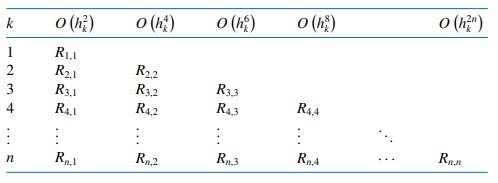
\includegraphics[width=0.65\linewidth]{TableR.JPG}}
\caption{Matrix Methods}
\label{RR}
\end{figure}
\begin{lstlisting}
%Romberg
fun = @(x) sin(x); %input the function
er = 0.00002; %give the error bound
a = 0;
b = pi;
n = 6;
R = zeros(2,n);
h = b-a;
R(1,1) = h*( fun(a) + fun(b) ) / 2;
RR = zeros(n,n);
RR(1) = R(1,1);
for i = 2 : n
    sum = 0;
    for k = 1 : 2^(i-2)
        sum = sum + fun(a+(k-0.5)*h);
    end
    R(2,1) = ( R(1,1) + h*sum ) / 2;
    for j = 2 : i
        R(2,j) = R(2,j-1) + ( R(2,j-1)-R(1,j-1) ) / ( 4^(j-1) - 1 );
    end
    h = h / 2;
    R(1,1:i) = R(2,1:i);
    RR(i,1:i) = R(2,1:i);
end
RR
\end{lstlisting}
Then we could get the final matrix as follows and the value that we calculate is the same as the one shown in the book.
\begin{table}[!ht]
    \centering
    \resizebox{\textwidth}{!}{
    \begin{tabular}{|c|c|c|c|c|c|c|}
    \hline
        \textbf{k} & \textbf{O(h2)} & \textbf{O(h4)} & \textbf{O(h6)} & \textbf{O(h8)} & \textbf{O(h10)} & \textbf{O(h12)} \\ \hline
        \textbf{1} & 1.92367069372179e-16 & 0 & 0 & 0 & 0 & 0 \\ \hline
        \textbf{2} & 1.57079632679490 & 2.09439510239320 & 0 & 0 & 0 & 0 \\ \hline
        \textbf{3} & 1.89611889793704 & 2.00455975498442 & 1.99857073182384 & 0 & 0 & 0 \\ \hline
        \textbf{4} & 1.97423160194555 & 2.00026916994839 & 1.99998313094599 & 2.00000554997967 & 0 & 0 \\ \hline
        \textbf{5} & 1.99357034377234 & 2.00001659104794 & 1.99999975245457 & 2.00000001628804 & 1.99999999458729 & 0 \\ \hline
        \textbf{6} & 1.99839336097014 & 2.00000103336941 & 1.99999999619084 & 2.00000000005967 & 1.99999999999603 & 2.00000000000132 \\ \hline
    \end{tabular}
    }
    \caption{Romberg Matrix}
    \label{RR}
\end{table}

\subsection{Gaussian Quadrature on Arbitrary Intervals}
Gaussian method has the same method shown before.Suppose that $x_1$, $x_2$, ... , $x_n$ are the roots of the nth Legendre polynomial $P_n(x)$ and that for
each $i$ = 1, 2, ... , n, the numbers $c_i$ are defined by
\begin{align}
    c_{i}=\int_{-1}^{1} \prod_{\substack{j=1 \\ j \neq i}}^{n} \frac{x-x_{j}}{x_{i}-x_{j}} d x\nonumber
\end{align}
If P(x) is any polynomial of degree less than 2n, then
\begin{align}
    \int_{-1}^{1} P(x) d x=\sum_{i=1}^{n} c_{i} P\left(x_{i}\right)\nonumber
\end{align}
For the normal kinds of the intervals we make $x = \frac{b+a+(b-a)s}{2}$have the changing form as follows
\begin{align}
    I=\int_{a}^{b} f(x) d x &=\int_{-1}^{1} f\left(\frac{b+a+(b-a) s}{2}\right) \times \frac{b-a}{2} d s \nonumber\\
&=\frac{b-a}{2} \Sigma_{i=1}^{m} c_{i} f\left(\frac{b+a+(b-a) s_{i}}{2}\right)\nonumber
\end{align}
Then we could calculate the intervals with the given constants 
\begin{lstlisting}
%Guasian Quadrature on Arbitrary Intervals
fun = @(x) sin(x); %input the function
er = 0.00002; %give the error bound
a = 0;
b = pi;
%  setup the gauss data
for n = 2:4
    if n == 2
        s = [-1 1]/sqrt(3);
        A = [1 1];
    elseif n == 3
        s = [-sqrt(3/5) 0 sqrt(3/5)];
        A = [5 8 5]/9;
    elseif n == 4
        s = [   -sqrt((15+2*sqrt(30))/35),  -sqrt((15-2*sqrt(30))/35), ...
            sqrt((15-2*sqrt(30))/35),   sqrt((15+2*sqrt(30))/35)];
        A = [  (90-5*sqrt(30))/180,    (90+5*sqrt(30))/180,...
            (90+5*sqrt(30))/180,    (90-5*sqrt(30))/180];
    end
    n
    xx = ( a+b+(b-a)*s ) / 2;
    I_sum = 0;
    for i = 1 : n
        I_sum = I_sum + A(i).*fun(xx(i));
    end
    I = I_sum*(b-a)/2
end
\end{lstlisting}
And we get the table as follows which shows the relations between the n and Intervals 
\begin{table}[!ht]
    \centering
    \begin{tabular}{|c|c|}
    \hline
        \textbf{n} & \textbf{Intervals} \\ \hline
        \textbf{2} & 1.935819575 \\ \hline
        \textbf{3} & 2.001388914 \\ \hline
        \textbf{4} & 1.999984228 \\ \hline
    \end{tabular}
    \caption{Gaussian Quadrature}
    \label{GAU}
\end{table}

\subsection{Compare of the methods}
To compare these methods we use the function $e^x$ and calculate the integration of it on [0,4],the code are as follows
\begin{lstlisting}
%Comepare the Integration methods
fun = @(x) exp(x);
a = 0;
b = 4;
Ireal = exp(4) - 1;

(b-a) / ((0.0001/(exp(4))*180/4)^0.25) - 2
(b-a) / ((0.0001/(exp(1))*180/4)^0.25) - 2


IRom(fun,a,b,6)
[I,B] = IGua(fun,a,b);
I

n = 0;
re = 1;
while re > 0.0001
    n = n+1;
    nn = n*2;
    I = ISim(fun,a,b,nn);
    re = I(nn-1) - Ireal;
end
nn
ISim(fun,a,b,nn) - Ireal*ones(1,nn-1)
IRom(fun,a,b,6) - Ireal*ones(6,6)
[I,B] = IGua(fun,a,b);
I - Ireal*ones(3,1)
\end{lstlisting}
In this part we first calculate the n in Simpson which is 30.Then we calculate all the results.
\begin{table}[!ht]
    \centering
    \begin{tabular}{|c|c|c|}
    \hline
        \textbf{Method} & \textbf{Intervals} & \textbf{error} \\ \hline
        \textbf{Simpson(n=30)} &   53.598243943577010  &      9.391043277418021e-05  \\ \hline
        \textbf{Romberg} &   53.598150733014634  &      6.998703980798382e-07  \\ \hline
        \textbf{Gaussian(n=2)} &   51.549379834805336  &   -2.048770198338900  \\ \hline
        \textbf{Gaussian(n=3)} &   53.530348665418813  &   -0.067801367725423  \\ \hline
        \textbf{Gaussian(n=4)} &   53.596948200324462  &   -0.001201832819774  \\ \hline
    \end{tabular}
    \caption{Compare of the methods}
    \label{COM2}
\end{table}
Then we could see that for the same function Romberg Method has the closest Intervals values.
\newpage
\section*{Appendix}
\addcontentsline{toc}{section}{Appendix}
\subsection*{Forward/Backward-Difference}
\lstinputlisting{FBdiff.m}
\subsection*{Three-Point Endpoint Difference}
\lstinputlisting{P3End.m}
\subsection*{Three-Point Midpoint Difference}
\lstinputlisting{P3Mid.m}
\subsection*{Five-Point Endpoint Difference}
\lstinputlisting{P5End.m}
\subsection*{Five-Point Midpoint Difference}
\lstinputlisting{P5Mid.m}
\subsection*{Composite Simpson's Rule}
\lstinputlisting{ISim.m}
\subsection*{Romberg}
\lstinputlisting{IRom.m}
\subsection*{Gaussian Quadrature}
\lstinputlisting{IGua.m}
\end{document}





